\documentclass[class=report, crop=false]{standalone}
\usepackage{msc_thesis}
\usepackage{wrapfig}

%!TeX spellcheck = en-GB

\begin{document}

\chapter{Theory}%
\label{chap:Theory}

\section{Classical Electrodynamics}
\label{sect:classical-electrodynamics}

{\color{red} Introduction stuff, cite~\textcite{eisenberg_nucleartheory_1978,jackson_classicalelectrodynamics_1999}}.

We will begin with Maxwell's equations in free space
\begin{subequations}%
  \label{eq:maxwell}
  \begin{align}
    \div{\vb{E}} & = \frac{\rho}{\varepsilon_0} \label{eq:coulomb-law} \\
    \div{\vb{B}} & = 0 \label{eq:gauss-law} \\
    \curl{\vb{E}} & = - \pdv{\vb{B}}{t} \label{eq:faraday-law} \\
    \curl{\vb{B}} & = \mu_0 \vb{j} + \frac{1}{c^2} \pdv{\vb{E}}{t} \,, \label{eq:ampere-law}
  \end{align}
\end{subequations}

which relate the electromagnetic field to sources, which must satisfy an additional
equation to ensure charge conservation
\begin{equation}
  \label{eq:continuity-equation}
  \div{\vb{j}(\vb{r}, t)} + \pdv{\rho(\vb{r}, t)}{t} = 0 \,.
\end{equation}

As we can see above, equations~\eqref{eq:faraday-law} and~\eqref{eq:gauss-law}
do not involve sources and thus they state the dynamical properties of the fields.
Since equations~\eqref{eq:coulomb-law} and~\eqref{eq:ampere-law} describe how
the sources influence the fields, we need an additional equation to describe how
the fields affect the sources
\[
  \vb{F} = \int \dd{\vb{r}'} \rho(\vb{r}', t) \vb{E}(\vb{r}', t) +
           \frac{1}{c} \int \dd{\vb{r}'} \vb{j}(\vb{r}', t) \cross \vb{B}(\vb{r}', t)\,.
\]

Maxwell's equations~\eqref{eq:maxwell} relate six field quantities (\(\vb{E}\) and \(\vb{B}\))
to four source quantities (\(\rho\) and \(\vb{j}\)). This implies that there are some
restrictions on the six quantities. This suggets that we can find a less redundant
way to express the fields, and indeed the four quantities given by the
vector potential \(\vb{A}\) and scalar potential \(\rho\) provide this representation.
Equation~\eqref{eq:gauss-law} implies the existence of a vector potential
\begin{equation}
  \label{eq:vector-potential}
  \vb{B}(\vb{r}, t) = \curl{\vb{A}(\vb{r}, t)}\,.
\end{equation}

Substituting~\eqref{eq:vector-potential} in~\eqref{eq:faraday-law} we obtain
\begin{equation}
  \label{eq:faraday-vector-potential}
  \curl(\vb{E} + \pdv{\vb{A}}{t}) = 0
\end{equation}

and thus the quantity in the paranthesis can always be expressed as the
gradient of a scalar field, namely the scalar potential
\[
\grad{\phi}(\vb{r}, t) = -\vb{E}(\vb{r}, t) - \pdv{\vb{A}}{t}\,.
\]

With these considerations~\eqref{eq:coulomb-law} becomes
\[
  \div(\grad{\phi} + \pdv{\vb{A}}{t}) = - \frac{\rho}{\varepsilon_0}
\]
or
\begin{equation}
  \label{eq:coulomb-scalar-potential}
  \laplacian{\phi} + \pdv{t}\div{\vb{A}} = - \frac{\rho}{\varepsilon_0}
\end{equation}

and~\eqref{eq:ampere-law}

\begin{equation}
  \label{eq:ampere-potentials-pre}
  \curl(\curl{\vb{A}}) = \mu_0 \vb{j}
    - \frac{1}{c^2} \pdv{t} \left( \grad{\phi} + \pdv{\vb{A}}{t} \right)\,.
\end{equation}

Using the following vector identity
\begin{equation}
  \label{eq:curl-of-curl}
  \curl(\curl{\vb{A}}) = \grad(\div{\vb{A}}) - \laplacian{\vb{A}}
\end{equation}

eq.~\eqref{eq:ampere-potentials-pre} becomes
\[
  \grad(\div{\vb{A}}) - \laplacian{\vb{A}} = \mu_0 \vb{j}
    - \frac{1}{c^2} \left( \grad{\pdv{\phi}{t}} + \pdv[2]{\vb{A}}{t} \right)
\]
or
\begin{equation}
  \label{eq:ampere-potentials}
  \laplacian{\vb{A}} - \frac{1}{c^2}\pdv[2]{\vb{A}}{t} =
    -\mu_0 \vb{j} + \grad(\div{\vb{A}} + \frac{1}{c^2} \pdv{\phi}{t})\,.
\end{equation}

Equations~\eqref{eq:coulomb-scalar-potential} and~\eqref{eq:ampere-potentials}
were obtained by substituting the potentials obtained from the source-less
equations,~\eqref{eq:gauss-law} and~\eqref{eq:faraday-law}, into the ones
with sources,~\eqref{eq:coulomb-law} and~\eqref{eq:ampere-law}. They are thus
fully equivalent with Maxwell's equations~\eqref{eq:maxwell} and, as we can observe,
relate the four quantities given by the potentials to the four quantities for the
sources. They also preserve the invariance under Lorentz transformations, with
the scalar potential \(\phi\) as the time-like component.

Equations~\eqref{eq:coulomb-scalar-potential} and~\eqref{eq:ampere-potentials}
can be simplified by decoupling the potentials. This is possible due to the fact
that potentials are not unique. To illustrate this point consider
\[
  \vb{A}'(\vb{r},t) = \vb{A}(\vb{r},t) + \grad{\Lambda}(\vb{r},t)\,.
\]

This vector potential gives rise to a magnetic field
\[
  \curl{\vb{A}'} = \curl{\vb{A}} + \curl(\grad{\Lambda}) = \curl{\vb{A}} = \vb{B}
\]
equal with the original one since \( \curl(\grad{\varphi}) = 0 \).

Similarly, for a scalar potential
\[
  \phi'(\vb{r},t) = \phi(\vb{r},t) - \pdv{\Lambda(\vb{r},t)}{t}
\]
and the corresponding electric field will be
\[
  - \grad{\phi'} - \pdv{\vb{A'}}{t} =
  - \grad{\phi} + \grad{\pdv{\Lambda}{t}} - \pdv{\vb{A}}{t} - \pdv{t} \grad{\Lambda}
  = - \grad{\phi} - \pdv{\vb{A}}{t}
  = \vb{E}\,,
\]
since the spatial and temporal derivatives commute. These kinds of transformations
are called gauge transformations.

\subsection{Gauge transformations}

The freedom of choosing the gauge leads to the following condition satisfied by
the scalar and vector potentials
\[
  \div{\vb{A}} + \frac{1}{c^2}\pdv{\phi}{t} = 0\,,
\]
called the Lorenz condition.

Indeed, if we consider a set of potentials \(\vb{A}\) and \(\phi\) that
don't satisfy the condition
\[
  \div{\vb{A}} + \frac{1}{c^2}\pdv{\phi}{t} \ne 0 = f(\vb{r},t)\,,
\]
then we can always carry out a gauge transformation to a new set of potentials
\(\vb{A}'\) and \(\phi'\) that satisfy the Lorenz condition, such that
\begin{align*}
  \div{\vb{A}} + \frac{1}{c^2}\pdv{\phi}{t} &= \div(\vb{A}' - \grad{\Lambda})
    + \frac{1}{c^2}\pdv{t} \left( \phi' + \pdv{\Lambda}{t} \right) \\
    &= \div{\vb{A}'} - \laplacian{\Lambda} + \frac{1}{c^2}\pdv{\phi'}{t}
    + \frac{1}{c^2}\pdv[2]{\Lambda}{t}
    = f(\vb{r},t)
\end{align*}

or
\[
  \div{\vb{A}} + \frac{1}{c^2}\pdv{\phi}{t} =
  \dalambert \Lambda \equiv \frac{1}{c^2}\pdv[2]{\Lambda}{t} - \laplacian{\Lambda} = f(\vb{r},t)\,,
\]

where the d'Alambertian operator is defined as
\[
  \dalambert \equiv \frac{1}{c^2}\pdv[2]{t} - \laplacian
\]
when choosing the Minkowski metric \( (+,-,-,-) \) and
\[
  \div{\vb{A'}} + \frac{1}{c^2}\pdv{\phi'}{t} = 0\,,
\]
since they satisfy the Lorenz condition.
The transformation we need is thus defined by the solution of \(\dalambert \Lambda = f\).

Imposing the Lorenz condition on equations~\eqref{eq:coulomb-scalar-potential}
and~\eqref{eq:faraday-vector-potential} decouples the potentials
\begin{align*}
  \laplacian{\phi} - \pdv{t} \frac{1}{c^2} \pdv{\phi}{t} = -\frac{\rho}{\varepsilon_0} \\
  \laplacian{\vb{A}} - \frac{1}{c^2}\pdv[2]{\vb{A}}{t} = -\mu_0 \vb{j}
\end{align*}
yielding the simplified form of Maxwell's equations
\begin{align*}
  \dalambert \phi &= \frac{\rho}{\varepsilon_0} \\
  \dalambert \vb{A} &= \mu_0 \vb{j}\,.
\end{align*}

This form of Maxwell's equations preserves Lorentz invariance, as the Lorenz
gauge condition can be expressed in a covariant way as the contraction of the
four-vector \(A \equiv (\frac{\phi}{c}, \vb{A})\) with the four-gradient
\((\frac{1}{c}\pdv{t}, -\grad)\).

Since the Lorenz condition doesn't fix the gauge, but only restricts us to
transformations with \(\dalambert \Lambda = 0\), we can impose further conditions
in order to fix the gauge, but in general those will not be covariant.
One such condition is given by the Coulomb gauge
\begin{equation}
  \label{eq:coulomb-gauge}
  \div{\vb{A}} = 0.
\end{equation}

In this gauge eq.~\eqref{eq:coulomb-scalar-potential} becomes a Poisson equation
for the scalar potential
\begin{equation}
  \label{eq:coulomb-poisson}
  \laplacian{\phi} = -\frac{\rho}{\varepsilon_0}
\end{equation}
with the solution given by the instantaneous Coulomb potential of the charge
density in the domain \(\rho(\vb{r},t)\)
\begin{equation}
  \label{eq:scalar-potential-solution}
  \phi(\vb{r},t) = \frac{1}{4\pi \varepsilon_0} \int \frac{\rho(\vb{r}',t)}{|\vb{r}-\vb{r}'|} \dd{\vb{r}}'\,,
\end{equation}
explaining the name of the condition~\eqref{eq:coulomb-gauge}.

An apparent violation of special relativity shows up in the above result which
states that the scalar potential (at time \(t\)) is given by the instantaneous Coulomb
interactions between charges (also at time \(t\)). The contradiction is only
apparent and stems from the act that the Coulomb gauge is not Lorentz invariant.

In order to resolve the contradiction we first note that we can only observe
the electric field
\[
  \vb{E}(\vb{r}, t) = -\grad{\phi}(\vb{r},t) -\pdv{\vb{A}(\vb{r},t)}{t}\,.
\]
Thus, the instantaneous propagation is removed by the time derivative
of the vector potential.

In the Coulomb gauge, the vector potential is given by
\begin{equation}
  \label{eq:vector-potential-coulomb-gauge}
  \dalambert \vb{A} = \mu_0 \vb{j} - \frac{1}{c^2} \grad{\pdv{\phi}{t}}\,.
\end{equation}

Considering the continuity equation~\eqref{eq:continuity-equation} and
the form of the scalar potential in eq.~\eqref{eq:scalar-potential-solution},
the second term in eq.~\eqref{eq:vector-potential-coulomb-gauge} becomes
\begin{equation}
  \label{eq:scalar-potential-continuity-equation}
  \grad{\pdv{\phi}{t}} = \grad \frac{1}{4\pi \varepsilon_0}
    \int \frac{\pdv{\rho}{t}}{|\vb{r}-\vb{r}'|} \dd{\vb{r}}'
    = - \frac{1}{4\pi \varepsilon_0} \grad
    \int \frac{\boldsymbol{\nabla}' \vdot \vb{j}(\vb{r}',t)}{|\vb{r}-\vb{r}'|} \dd{\vb{r}}'\,,
\end{equation}
where \(\boldsymbol{\nabla}'\) denotes the derivatives with respect to \(\vb{r}'\).
Using the Helmholz decomposition we can write any sufficiently well behaved
vector (the current density in this particular case) as the sum
of a divergence-free (transversal) component and a curl-free (longitudinal) one:
\[
  \vb{j} = \vb{j}^t + \vb{j}^l \,,
\]
where
\begin{align*}
  \div{\vb{j}^t} &= 0 \\
  \curl{\vb{j}^l} &= 0 \,.
\end{align*}

Using the vector identity~\eqref{eq:curl-of-curl} and
\[
  \laplacian{\frac{1}{|\vb{r}-\vb{r}'|}} = -4\pi \delta(\vb{r}-\vb{r}')
\]
we can write the current density as follows
\begin{align*}
  \laplacian(\vb{j}^t + \vb{j}^l) &= \grad(\div{\vb{j}^l}) - \curl(\curl{\vb{j}^t}) \\
  \int \frac{\laplacian{\vb{j}}}{|\vb{r}-\vb{r}'|} \dd{\vb{r}} &=
    \int \frac{\grad(\div{\vb{j}^l})}{|\vb{r}-\vb{r}'|} \dd{\vb{r}'}
    - \int \frac{\curl(\curl{\vb{j}^t})}{|\vb{r}-\vb{r}'|} \dd{\vb{r}'} \\
  -4\pi \vb{j} &= \grad \int \frac{\div{\vb{j}^l}}{|\vb{r}-\vb{r}'|} \dd{\vb{r}'}
    - \curl \curl \int \frac{\vb{j^t}}{|\vb{r}-\vb{r}'|} \dd{\vb{r}'}
\end{align*}
and thus we obtain the two components as

\begin{align*}
  \vb{j}^t &= \frac{1}{4\pi} \curl \curl \int \frac{\vb{j}(\vb{r}',t)}{|\vb{r}-\vb{r}'|} \dd{\vb{r}}' \\
  \vb{j}^l &= -\frac{1}{4\pi} \grad \int
    \frac{\boldsymbol{\nabla}' \vdot \vb{j}(\vb{r}',t)}{|\vb{r}-\vb{r}'|} \dd{\vb{r}}'\,.
\end{align*}

Comparing with~\eqref{eq:scalar-potential-continuity-equation} we see that
\[
  \frac{1}{c^2} \grad{\pdv{\phi}{t}} = \frac{\varepsilon_0}{c^2} \vb{j}^l
  = \mu_0 \vb{j}^l
\]
and thus the source term in eq.~\eqref{eq:vector-potential-coulomb-gauge} can
be expressed as function of the transverse current:
\[
  \dalambert \vb{A} = \mu_0 (\vb{j} - \vb{j}^l) = \mu_0 \vb{j}^t\,
\]
and this also why the Coulomb gauge is also called the transverse gauge.
This gauge is useful when no sources are present. In this case \(\phi=0\),
\(\vb{A}\) satisfies the homogenuous wave equation and the fields can
be expressed only as function of the vector potential
\begin{align*}
  \vb{E} &= -\pdv{\vb{A}}{t} \\
  \vb{B} &= \curl{\vb{A}}\,.
\end{align*}

\subsection{The Poynting theorem}

In order to complete the description of the interaction between fields
and sources, we will now focus on how the fields affect the particles.
We begin by considering the force acting on a charge \(q\)
\[
  \vb{F} = q\vb{E} + q\vb{v} \cp \vb{B}\,.
\]

The corresponding infinitezimal variation of the force is given by
\[
  \var{\vb{F}} = \rho \vb{E} \var{V} + \vb{j} \cp \vb{B} \var{V}
    = (\rho \vb{E} + \vb{j} \cp \vb{B}) \var{V}
    \equiv f \var{V},
\]
where \(f = \rho \vb{E} + \vb{j} \cp \vb{B}\) is the Lorentz force
density. We can now consider a uniform charge distribution characterized
by \(\rho\). For an infinitezimal volume \(\var{V}\) of this charge distribution,
the rate of change of the work, or the power given by the
fields is given by
\[
  \vb{v} \vdot \vb{F} = \rho \vb{v} \vb{E} + \frac{\vb{j}}{q} \vdot (\vb{j} \cp \vb{B})
    = \rho \vb{v} \vb{E}\,.
\]

As we can see above, the magnetic force doesn't contribute to the work
done by the fields. Thus, the power transferred from the fields to the
charges in a finite domain \(\mathscr{D}\) is
\[
  \int_{\mathscr{D}} \vb{j} \vdot \vb{E} \dd{\vb{r}}\,.
\]

For the energy to conserve, this power must be balanced by a corresponding
rate of decrease of energy in the electromagnetic field.
Using the Ampère law~\eqref{eq:ampere-law}
\[
  \int_{\mathscr{D}} \vb{j} \vdot \vb{E} \dd{\vb{r}} =
  \int_{\mathscr{D}} \vb{E} \vdot \frac{1}{\mu_0} \qty(\curl{\vb{B}} - \frac{1}{c^2} \pdv{\vb{E}}{t}) \dd{\vb{r}} =
  \frac{1}{\mu_0} \int_{\mathscr{D}} \left[\vb{E} \vdot(\curl{\vb{B}}) -
    \frac{1}{c^2} \vb{E} \vdot \pdv{\vb{E}}{t} \right] \dd{\vb{r}}
\]

Using the following vector identity
\[
  \div(\vb{E} \cp \vb{B}) = \vb{B} \vdot (\curl{E}) - \vb{E} \vdot (\curl{\vb{B}})
\]
we can express \(\vb{E} \vdot(\curl{\vb{B}})\) as
\[
  \vb{E} \vdot(\curl{\vb{B}}) = \vb{B} \vdot (\curl{E}) - \div(\vb{E} \cp \vb{B}) =
  - \vb{B} \vdot \pdv{\vb{B}}{t} - \div(\vb{E} \cp \vb{B})\,,
\]
where we used~\eqref{eq:faraday-law} for the first term.

Using this result, the power transferred by the fileds is given by
\[
  \int_{\mathscr{D}} \vb{j} \vdot \vb{E} \dd{\vb{r}} =
  -\int_{\mathscr{D}} \left[\frac{1}{\mu_0} \div(\vb{E} \cp \vb{B}) + \frac{1}{\mu_0} \vb{B} \vdot \pdv{\vb{B}}{t} +
    \frac{1}{\mu_0 c^2} \vb{E} \vdot \pdv{\vb{E}}{t} \right] \dd{\vb{r}}
\]

Considering that
\[
  \vb{E} \vdot \pdv{\vb{E}}{t} = \frac{1}{2} \pdv{t} \vb{E}^2\,,
\]
we obtain
\[
  \int_{\mathscr{D}} \vb{j} \vdot \vb{E} \dd{\vb{r}} =
  -\int_{\mathscr{D}} \left[ \frac{1}{2} \pdv{t}
    \left( \varepsilon_0 \vb{E}^2 + \frac{1}{\mu_0}\vb{B}^2 \right)
  + \frac{1}{\mu_0}\div(\vb{E} \cp \vb{B}) \right] \dd{\vb{r}}\,.
\]

The total energy density of the electromagnetic field can be denoted wity
\[
  w_{em} = \frac{1}{2} \left( \varepsilon_0 \vb{E}^2 + \frac{1}{\mu_0}\vb{B}^2 \right)
\]
and thus we obtain
\[
  -\int_{\mathscr{D}} \vb{j} \vdot \vb{E} \dd{\vb{r}} =
  \int_{\mathscr{D}} \left[ \pdv{w_{em}}{t} +
  \frac{1}{\mu_0}\div(\vb{E} \cp \vb{B}) \right] \dd{\vb{r}}\,.
\]

Since the domain \(\mathscr{D}\) is arbitrary, we can write the above as a
differential continuity equation
\begin{equation}
  \label{eq:poynting-theorem-local}
  \pdv{w_{em}}{t} = - \div{\vb{S}} - \vb{j} \vdot \vb{E}\,,
\end{equation}
where
\[
  \vb{S} = \frac{1}{\mu_0} \vb{E} \cp \vb{B}
\]
is the Poynting vector representing the energy flow.

If we consider the domain \(\mathscr{D}\) such that no particles will leave it
\[
  W_{em} = \int_{\mathscr{D}} w_{em} \dd{\vb{r}}
\]
is the energy of the electromagnetic field and \(W_{mech}\) is the
energy of the particles
\[
  W_{mech} = \int_{\mathscr{D}} w_{mech} \dd{\vb{r}} =
  \int_{\mathscr{D}} \vb{j} \vdot \vb{E} \dd{\vb{r}}\,.
\]

By using Gauss' theorem, the energy flux corresponding to the
Poynting vector becomes
\[
  \int_{\mathscr{D}} \div{\vb{S}} = \oint_\Sigma \vb{n} \vdot \vb{S} \dd{a}\,,
\]
where \(\Sigma\) is the surface enclosing the domain \(\mathscr{D}\).

With the above considerations Poynting's theorem gives the conservation of energy for the whole system
\begin{equation}
  \label{eq:poynting-theorem}
  \dv{W}{t} = \dv{t} \left( W_{em} + W_{mech} \right) =
  -\oint_\Sigma \vb{n} \vdot \vb{S} \dd{a}\,,
\end{equation}

stating that the rate of change of the energy of the system composed of the charged
particles and corresponding fileds is given by minus the flux of the
Poynting vector through the surface bounding the domain.

Equation~\eqref{eq:poynting-theorem-local} is the local form for the Poynting
theorem.

If we consider the extension of the domain to infinity \(\mathscr{D} \to \mathbb{R}^3\),
\(\Sigma \to \Sigma_\infty\), then there is no energy flow through the
boundary since electromagnetic waves propagate at a constant finite speed \(c\). Then
\[
  \dv{W}{t} = \dv{t} \left( W_{em} + W_{mech} \right) = 0
\]
and the entire energy of the electromagnetic field can be converted into
the mechanical energy of the particles interacting with the field.

If we consider \(\mathscr{D}\) such that it doesn't enclose any sources, than
\[
  \dv{t} W_{em} = -\oint_\Sigma \vb{n} \vdot \vb{S} \dd{a}\,,
\]
which shows that the energy of the electromagnetic field in the domain
\(\mathscr{D}\) can change through the variation of the flux of the
Poynting vector on the boundary of the domain, \(\Sigma\). Thus we can
indeed say that the flux of the Poynting vector is the energy flux.

\subsection{Electromagnetic waves}


\section{Electron in a Plane Wave}

In this section we will consider the classical dynamics of an electron in a
laser pulse following the discusion in~\textcite{karsch_applicationshigh_2018}.
The starting point is the equation of motion for the electron
\begin{equation}
  \label{eq:lorentz-eom}
  \dv{\vb{p}}{t} = -e \left[ \vb{E}(\vb{r}, t) + \vb{v} \cp \vb{B}(\vb{r}, t) \right]\,.
\end{equation}

\subsection{Non-relativistic treatment}

\subsection{Relativistic treatment}

\section{Particle in Cell Method}

As we outlined in section~\ref{sect:classical-electrodynamics}, the interaction
of some charged particles with an electromagnetic field can be viewed as the
action of the sources on the fields and the action of the fields on the sources.

In the same manner, simulating the interaction self-consistently rquires a
\emph{field solver} that computes the structure of the fields considering
the sources and a \emph{particle pusher} that solves the (relativistic)
equations of motion for the particles.
In the particle in cell method, a finite-difference time-domain (FDTD) method
is used for solving Maxwell's equations and a modified leapfrog method is used
for the particle pusher as presented in~\cite{arber_contemporaryparticleincell_2015}.

\subsection{Discretizations}

The numerical methods mentioned above are based on the idea of discretizing the
derivative operator. There are multiple ways of discretizing this operator,
but all of them can be derived from the Taylor series expansion.
\[
  f(x_0+h) = f(x_0) + \frac{f'(x_0)}{1!}h + \frac{f''(x_0)}{2!}h^2 + \dotsb + \frac{f^{(n)}(x_0)}{n!}h^n + \dots
\]

The main discretizations options are the forward, backward and central differences.
For the forward discretization we consider
\[
  f(x_0+h) = f(x_0) + \frac{f'(x_0)}{1!}h + \frac{f''(x_0)}{2!}h^2 + \dotsb
\]
and we rearange the terms in the following way
\[
  \frac{f(x_0+h) - f(x_0)}{h} = f'(x_0) + \frac{f''(x_0)}{2}h + \dotsb
\]
and thus, when \(h \to 0\), the derivative in first order is given by
\[
  f'(x_0) = \frac{f(x_0+h) - f(x_0)}{h} + \order{h}\,.
\]

The local truncation error is given by the error of the approximation in one time
step. The forward and backward discretizations are both of order one. The
central discretization is second order accurate and can be derived as follows.

We first begin with the forward and backward discretizations for half of a
timestep:
\begin{align*}
  f(x_0+\frac{h}{2}) &= f(x_0) + f'(x_0)\frac{h}{2} + \frac{f''(x_0)}{2}\frac{h^2}{4}
    + \frac{f^{(3)}(x_0)}{3!}\frac{h^3}{8} + \dotsb \\
  f(x_0-\frac{h}{2}) &= f(x_0) - f'(x_0)\frac{h}{2} + \frac{f''(x_0)}{2}\frac{h^2}{4}
    - \frac{f^{(3)}(x_0)}{3!}\frac{h^3}{8} + \dotsb \,.
\end{align*}

Then we take the difference and obtain
\[
  f(x_0+\frac{h}{2}) - f(x_0-\frac{h}{2}) = f'(x_0)h
    + 2\frac{f^{(3)}(x_0)}{3!}\frac{h^3}{8} + \dotsb
\]
and we can see that indeed the centeral diference is second order accurate
\[
  f'(x_0) = \frac{f(x_0+\frac{h}{2}) - f(x_0-\frac{h}{2})}{h} + \order{h^2}\,.
\]

As an application of the methods discussed above, we will now derive the so called
leapfrog method for solving second order differential equations
following~\textcite[Chapter~4]{hockney_computersimulation_1988}. More concretely,
we will take a look at solving the equations of motion for a particle. As a first
step, the equations of motion can be written as a system of first order differential
equations
\begin{align*}
  \dv{\vb{x}}{t} &= \vb{v} \\
  m \dv{\vb{v}}{t} &= \vb{F}\,,
\end{align*}
where \(\vb{F}\) is the total force on the particle. Replacing the derivatives
with their finite difference approximations, we obtain
\begin{align*}
  \frac{\vb{x}_{n+1} - \vb{x}_n}{\Delta t} = \vb{v}_{n+1/2} \\
  m \frac{\vb{v}_{n+1/2} - \vb{v}_{n-1/2}}{\Delta t} = \vb{F}(\vb{x}_n)\,.
\end{align*}
Replacing the velocity, we obtain
\begin{equation}
  \label{eq:leapfrog}
  \frac{\vb{x}_{n+1}-2\vb{x}_n+\vb{x}_{n-1}}{\Delta t^2} = \frac{\vb{F}(\vb{x}_n)}{m}\,.
\end{equation}

\subsubsection{Accuracy}

The accuracy of an integration method is given by difference between the true
solution and the approximate solution at a given timestep, that is the local
error. There are two types of local errors: truncation errors and roundoff errors.
Truncation errors are given by the approximations employed in the numerical method.
On the other hand, roundoff errors are consequence of implementing the numerical
method on a computer with finite precision. In general, for low order methods,
the truncation errors are significantly bigger than roundoff errors, and thus
we can consider that the accuracy is given only by truncation error.

In order to better illustrate the concept of truncation errors, we will exemplify
its computation for the leapfrog method. Let us consider the local truncation
error at the timestep \(n\), \(\delta^n\) and \(\vb{X}\) the true solution
\[
  \frac{\vb{X}_{n+1}-2\vb{X}_n+\vb{X}_{n-1}}{\Delta t^2} = \frac{\vb{F}(\vb{X}_n)}{m} + \delta^n\,.
\]

If we expand \(\vb{X}_{n+1}\) and \(\vb{X}_{n-1}\) in Taylor series around \(\vb{X}_n\)
\begin{align*}
  \vb{X}_{n+1} &= \vb{X}_n + \dv{\vb{X}_n}{t}\Delta t + \frac{1}{2} \dv[2]{\vb{X}_n}{t} - \dotsb \\
  \vb{X}_{n-1} &= \vb{X}_n - \dv{\vb{X}_n}{t}\Delta t + \frac{1}{2} \dv[2]{\vb{X}_n}{t} - \dotsb\,,
\end{align*}
we obtain
\[
  \dv[2]{\vb{X}_n}{t} + \frac{\Delta t^2}{12} \dv[4]{\vb{X}}{t} + \order{\Delta t^5}
  = \frac{\vb{F}(\vb{X}_n)}{m} + \delta^n\,,
\]
and thus
\[
  \delta^n \sim \order{\Delta t^2}
\]
which shows that the leapfrog algorithm is of order 2.

\subsubsection{Stability}

A numerical method is considered asymptotically stable if the solution obtained
for a linear problem is asymptotically bounded.
As in the previous case we will show an example for the leapfrog method,
following the ideas exposed in~\cite{butcher_numericalmethods_2016}
and in~\textcite[Section 2.6]{leimkuhler_simulatinghamiltonian_2004}.

A linear problem can be written as
\[
\dv{t} \vb{z} = A \vb{z}\,,
\]
where we used the following notation to denote the dynamical state of the system
\[
\vb{z} =
\begin{pmatrix}
  \vb{q} \\
  \vb{p}
\end{pmatrix}\,.
\]

The solution can be written as
\begin{equation*}
  % \label{eq:linear-problem-solution}
  \vb{z}(t) = R(t) \vb{z}_0\,,
\end{equation*}
where \(R(t)\) is a matrix which can give the solution at any time by evolving
the initial conditions.

The discrete version of the problem is given by
\begin{equation}
  \label{eq:discrete-linear-problem}
  \vb{z}_{n+1} = \hat{R}(\Delta t) \vb{z}_n\,,
\end{equation}
where \(\hat{R}(\Delta t)\) is called the propagation matrix.
With this considerations, asymptotic stability can be expressed as a function
of the eigenvalues of \(\hat{R}(\Delta t)\), since the solution is obtained
with powers of \(\hat{R}\) from the initial conditions
\begin{equation*}
  % \label{eq:discrete-linear-solution}
  \vb{z}_n = [\hat{R}]^n \vb{z}_0\,.
\end{equation*}

More concretely, a method is asymptotically stable if the eigenvalues of
\(\hat{R}\) are inside the unit disk in the complex plane and simple (not repeated)
if on the unit circle~\autocite[28]{leimkuhler_simulatinghamiltonian_2004}.

One of the most studied linear problems is the harmonic oscillator and we can use
it as our model linear problem
\[
\mathcal{H} = \frac{\vb{p}^2}{2m} + \frac{\omega^2 \vb{q}^2}{2}\,.
\]

The equations of motion are given by the corresponding Hamilton equations
\begin{align*}
  \dot{q}_i &= \pdv{\mathcal{H}}{p_i} = \frac{p_i}{m} \\
  \dot{p}_i &= -\pdv{\mathcal{H}}{q_i} = -\omega^2 q_i\,.
\end{align*}

Taking \(m=1\) and writing the above equations in matrix form yields
\[
\dot{\vb{z}} =
\begin{pmatrix}
  p \\
  -\omega^2 q
\end{pmatrix} =
\begin{pmatrix}
  0 & 1 \\
  -\omega^2 & 0
\end{pmatrix}
\begin{pmatrix}
  \vb{q} \\
  \vb{p}
\end{pmatrix}
\]
and thus we obtain
\[
\dot{\vb{z}} = A \vb{z},
\]
with
\[
A =
\begin{pmatrix}
  0 & 1 \\
  -\omega^2 & 0
\end{pmatrix}\,.
\]

The solution is given by
\[
\vb{z}(t) = R(t) \vb{z}_0,
\]
with
\[
R(t) =
\begin{pmatrix}
  \cos(\omega t) & \frac{1}{\omega} \sin(\omega t) \\
  -\omega \sin(\omega t) & \cos(\omega t)
\end{pmatrix}\,.
\]

In order to analyze the stability of the leapfrog algorithm, it is convenient to
express the equations in a different form, also called the Störmer–Verlet method
\begin{align*}
  \vb{q}_{n+1} &= \vb{q}_n + \Delta t \vb{v}_{n+1/2} \\
  M \vb{v}_{n+1/2} &= M \vb{v}_n - \frac{\Delta t}{2} \grad{V(\vb{q}_n)} \\
  M \vb{v}_{n+1} &= M \vb{v}_{n+1/2} - \frac{\Delta t}{2} \grad{V(\vb{q}_{n+1})}\,.
\end{align*}

In our particular case, the gradient of the potential is given by
\(\omega^2 q\) and the above reduces to
\begin{align*}
  \vb{q}_{n+1} &= \vb{q}_n + \Delta t (\vb{v}_n - \frac{\Delta t}{2} \omega^2 \vb{q}^n) =
  \vb{q}_n \left(1 - \frac{\Delta t^2 \omega^2}{2}\right) + \vb{v}_n \Delta t \\
  \vb{p}_{n+1} &= \vb{p}_n - \frac{\Delta t^2}{2} \omega^2 \vb{q}_n
  -\frac{\Delta t^2}{2} \omega^2 \vb{q}_{n+1} =
  \vb{p}_n - \frac{\Delta t^2}{2} \omega^2 \vb{q}_n
  -\frac{\Delta t}{2}\omega^2 \left(\vb{q}_n+\vb{v}_n-\frac{\Delta t}{2}\omega^2 \vb{q}_n\right)\,,
\end{align*}
or
\[
\begin{pmatrix}
  \vb{q}_{n+1} \\
  \vb{p}_{n+1}
\end{pmatrix} =
\begin{pmatrix}
  1 - \frac{\Delta t^2 \omega^2}{2} & \Delta t \\
  -\Delta t \omega^2 \left(1 - \frac{\Delta t^2 \omega^2}{4}\right) &
  1 - \frac{\Delta t^2 \omega^2}{2}
\end{pmatrix}
\begin{pmatrix}
  \vb{q}_n \\
  \vb{p}_n
\end{pmatrix}\,.
\]

Comparing with~\eqref{eq:discrete-linear-problem} we obtain
\[
\hat{R}(\Delta t) =
\begin{pmatrix}
  1 - \frac{\Delta t^2 \omega^2}{2} & \Delta t \\
  -\Delta t \omega^2 \left(1 - \frac{\Delta t^2 \omega^2}{4}\right) &
  1 - \frac{\Delta t^2 \omega^2}{2}
\end{pmatrix}\,.
\]

The eigenvalues of \(\hat{R}\) are given by the solution of
\(
\det(\hat{R} - \lambda I) = 0
\), or more explicitly
\[
\vmqty{
1 - \frac{\Delta t^2 \omega^2}{2} & \Delta t \\
-\Delta t \omega^2 \left(1 - \frac{\Delta t^2 \omega^2}{4}\right) &
1 - \frac{\Delta t^2 \omega^2}{2}
} = 0\,.
\]

This reduces to
\[
\left(1-\frac{\Delta t^{2} \omega^2}{2}-\lambda\right)^{2}+
\frac{\Delta t^{2} \omega^2}{2}\left(2-\frac{\Delta t^2 \omega^2}{2}\right) = 0\,.
\]
Using the notation \(\frac{\Delta t^{2} w^{2}}{2}\equiv\mu^{2}\),
we obtain
\[
\left(1-\mu^{2}-\lambda\right)^2+\mu^{2}\left(2-\mu^{2}\right)=0\,,
\]
which can be further expanded to
\[
\lambda^{2}+\left(1-\mu^{2}\right)^{2}-2\left(1-\mu^{2}\right) \lambda+\mu^{2}\left(2-\mu^{2}\right)=0\,,
\]
yielding the solutions
\begin{align*}
  \lambda_{1,2} &= \frac{1}{2} \left\{2(1-\mu^2) \pm
  \sqrt{4(1-\mu^2)^2 - 4\left[(1-\mu^2)^2 + \mu^2 (2-\mu^2)\right]}\right\} \\
  &= 1-\mu^2 \pm \sqrt{\mu^2(\mu^2-2)}\,.
\end{align*}

We notice that for \(\mu^2 < 2\) the solutions are complex and
\begin{align*}
  |\lambda_{1,2}|^2 &= (1-\mu^2) + \mu^2 (\mu^2-2) \\
  &= 1+\mu^4-2\mu^2+\mu^4-2\mu^2 \\
  &= 1+\mu^4-4\mu^2\,.
\end{align*}

The method will be stable for \(|\lambda|^2 < 1\), or
\[
\mu^2 (\mu^2 - 4) < 0 \implies \mu < 2, \text{for } \mu \ne 0\,.
\]

For \(\mu^2 > 2\) the eigenvalues are real and with modulus greater than 1.
Thus the stability condition for the Störmer–Verlet method is given by \(\mu < 2\),
or
\[
\Delta t^2 \omega^2 < 4\,,
\]
indicating a sampling of at least \(\pi\) points per period, or a step size
\(\Delta t < 2/\omega\).

In the context of ordinary differential equations, a stability region of the method
can be defined via a stability function \(R(z)\) in the complex
plane~\autocite[81]{butcher_numericalmethods_2016}. Such approach cannot be used
in this case since the stability function is defined for a singe ordinary
differential equation, but in the case of Hamiltonian dynamics we always have
\(2n\) ordinary differential equations, with \(n>1\).

\subsection{The particle pusher}

Having (briefly) developed some general aspects of the theory of numerical methods
for solving differential equations, we now continue with the more concrete case
of numerically solving the equations of motion for a charged particle.
In the non-relativistic case, the (continuous) equations of motion have the
following form
\begin{align*}
  \dv{\vb{x}}{t} &= \vb{v} \\
  \dv{\vb{v}}{t} &= \frac{q}{m} \left(\vb{E} + \vb{v}\cp\vb{B}\right)\,.
\end{align*}

Since the above equations are symmetric with respect to time reversal, it is
desired that we obtain a discretization which is also time-reversible.
\Textcite{buneman_timereversibledifference_1967} explained that we can
use centered differences for this task and in the particular case of the
Lorentz force we can average the velocity in order to represent the
\(\vb{v} \cp \vb{B}\) product symmetrically. Thus we obtain
\begin{align}
  \label{eq:lorentz-discrete-x}
  \frac{\vb{x}_{n+1}-\vb{x}_n}{\Delta t} &= \vb{v}_{n+1} \\
  \label{eq:lorentz-discrete-v}
  \frac{\vb{v}_{n+1/2}-\vb{v}_{n-1/2}}{\Delta t} &= \frac{q}{m}
    \left(\vb{E}(\vb{x}_n) + \frac{\vb{v}_{n+1/2}-\vb{v}_{n-1/2}}{2} \cp \vb{B}(\vb{x}_n)\right)\,.
\end{align}

As explained in~\textcite[Chapter 4-3]{birdsall_plasmaphysics_2005}, there are
several methods for solving the above equations, implying a
partial~\autocite{buneman_timereversibledifference_1967} or
complete~\autocite{boris_relativisticplasma_1970} separation of the electric
and magnetic force contributions. In the following we will detail the second
method, which is also called the Boris push.

Let us introduce the following notation
\begin{align*}
  \vb{v}^- &= \vb{v}_{n-1/2} - \frac{q \vb{E}}{m} \frac{\Delta t}{2} \\
  \vb{v}^+ &= \vb{v}_{n+1/2} + \frac{q \vb{E}}{m} \frac{\Delta t}{2}\,,
\end{align*}
such that
\[
\frac{\vb{v}^+ - \vb{v}^-}{\Delta t} = \frac{\vb{v}_{n+1/2} - \vb{v}_{n-1/2}}{\Delta t}
+ \frac{q \vb{E}}{m}\,.
\]

Substituting in~\eqref{eq:lorentz-discrete-v} we obtain
\begin{equation}
  \label{eq:vp-vm-rotation}
  \frac{\vb{v}^+ - \vb{v}^-}{\Delta t} = \frac{q}{2m} (\vb{v}^+ + \vb{v}^-) \cp \vb{B}\,,
\end{equation}
which can be seen as a rotation. Indeed, if we take the scalar product with
\((\vb{v}^+ + \vb{v}^-)\), we get
\[
(\vb{v}^+ + \vb{v}^-) \vdot \frac{\vb{v}^+ - \vb{v}^-}{\Delta t} =
\frac{q}{2m} \underbrace{(\vb{v}^+ + \vb{v}^-) \vdot (\vb{v}^+ + \vb{v}^-) \cp \vb{B}}_{0}
\]
or
\[
|\vb{v}^+|^2 - |\vb{v}^-|^2 = 0\,,
\]
implying that \(|\vb{v}^+| = |\vb{v}^-|\).

If we decompose the \(\vb{v}^-\) into its parallel and perpendicular components
with respect to \(\vb{B}\), we can reduce the rotation of \(\vb{v}^-\) to
the rotation of its perpendicular component \(\vb{v}^-_\perp\).

\begin{wrapfigure}[12]{r}{0.4\textwidth}
  \centering
  \subimport{../figures/}{Boris-rotation-angle}%
  \caption{Boris rotation angle}\label{fig:Boris-rotation-angle}%
\end{wrapfigure}

The angle of rotation between \(\vb{v}^-_\perp\) and \(\vb{v}^-_\perp\),
denoted with \(\theta\) in figure~\ref{fig:Boris-rotation-angle},
can be expressed as
\[
\tan{\frac{\theta}{2}} = \frac{|\vb{v}^+_\perp - \vb{v}^-_\perp|}{|\vb{v}^+_\perp + \vb{v}^-_\perp|}\,.
\]

Rewriting eq.~\eqref{eq:vp-vm-rotation} we obtain
\[
\vb{v}^+ - \vb{v}^- = \frac{q \Delta t}{2m} (\vb{v}^+ + \vb{v}^-) \cp \vb{B}
\]
and if we substitute \(\vb{v}^\pm = \vb{v}^\pm_\perp + \vb{v}^\pm_\parallel\)
\[
\vb{v}^+_\perp - \vb{v}^-_\perp = \frac{q \Delta t}{2m} (\vb{v}^+_\perp + \vb{v}^-_\perp) \cp \vb{B}\,.
\]

Furthermore, since all the vectors above have the same direction by construction,
we can factor out the versors and obtain
\[
\frac{|\vb{v}^+_\perp - \vb{v}^-_\perp|}{|\vb{v}^+_\perp + \vb{v}^-_\perp|} =
\frac{q |\vb{B}|}{m} \frac{\Delta t}{2}
\]
and thus
\begin{equation}
  \label{eq:Boris-rotation-angle}
  \tan{\frac{\theta}{2}} = \frac{q B}{m} \frac{\Delta t}{2}\,.
\end{equation}

Since for the rotation described above only the components perpendicular to
the direction of \(\vb{B}\) matter, we can simplify the notation and use
\(\vb{v}_\pm\) instead of \(\vb{v}^\pm_\perp\).
We will now introduce an additional vector \(\vb{v}'\) given by the addition
between \(\vb{v}_-\) and another vector, such that \(\vb{v}'\) is perpendicular
to \(\vb{v}_+ - \vb{v}_-\).

It is convenient to write \(\vb{v}'\) as \(\vb{v}' = \vb{v}_- + \vb{v}_- \cp \vb{t}\).
In the right trinagle formed by \(\vb{v}'\) with \(\vb{v}_-\)
and \(\vb{v}_- \cp \vb{t}\) as seen in figure~\ref{fig:Boris-rotation-3D},
we have
\[
\tan{\frac{\theta}{2}} = \frac{|\vb{v}_- \cp \vb{t}|}{|\vb{v}_-|} = |\vb{t}|
\]
and thus by using eq.~\eqref{eq:Boris-rotation-angle} \(\vb{t}\) is given by
\[
\vb{t} = \frac{q \vb{B}}{m} \frac{\Delta t}{2}
\]

\begin{figure}[h]
  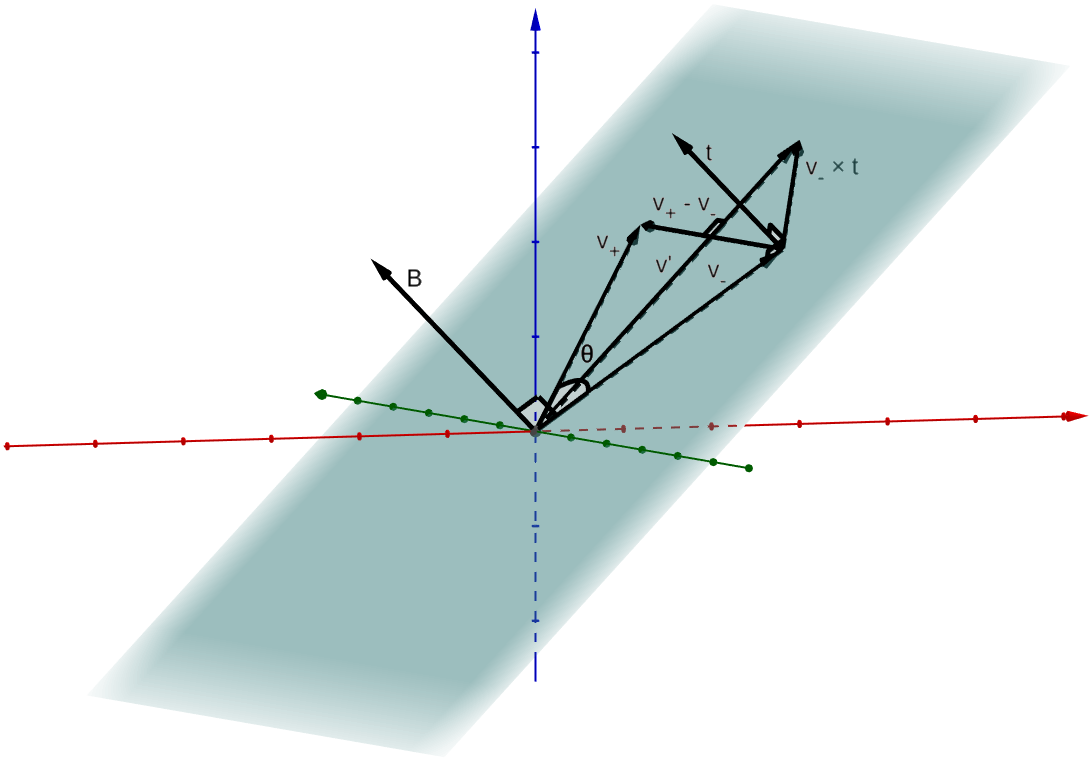
\includegraphics[width=\textwidth]{Boris-rotation-3D}
  \caption{Boris rotation construction in 3D}%
  \label{fig:Boris-rotation-3D}%
\end{figure}

\subsubsection{Conservation properties}

When solving (continuous) differential equations with (discrete) numerical methods,
an important aspect is that we want the algorithm to be as close as possible to
the original continuous system in terms of symmetries and conserved quantities.

In what follows we will look at the conservation properties of the Boris push
and show why are they important for simulating the dynamics of charged particles
following~\textcite{qin_whyboris_2013}.

\subsection{The field solver}

\subsection{A survey of available PIC codes}

\subsection{EPOCH}

\end{document}
